\documentclass{article}

\usepackage[tmargin=0.5in,bmargin=0.25in]{geometry}
\usepackage{amsmath, amssymb, amsthm}
\usepackage{listings}
\usepackage{multicol}
\usepackage{enumitem}
\usepackage{forest}
\usepackage{pdfpages}

\title{CSCI 305 Assignment 3}
\author{(Solo) Isaac Boaz}

\begin{document}
\maketitle

\begin{enumerate}
    \item Provide a \(\Theta\) bound for the solution of each of these recurrences.
          \begin{enumerate}[label=\arabic*.]
              \item \[T(n) = 7T(n/7) + n\]
                    \begin{center}
                        \begin{forest}
                            [$n$
                                [$\frac{n}{7}$
                                        [$\frac{n}{49}$]
                                            [$\frac{n}{49}$]
                                            [$\frac{n}{49}$]
                                            [$\frac{n}{49}$]
                                            [$\frac{n}{49}$]
                                            [$\frac{n}{49}$]
                                            [$\frac{n}{49}$]
                                    ]
                                    [$\frac{n}{7}$
                                        [$\vdots$]
                                    ]
                                    [$\frac{n}{7}$
                                        [$\vdots$]
                                    ]
                                    [$\frac{n}{7}$
                                        [$\vdots$]
                                    ]
                                    [$\frac{n}{7}$
                                        [$\vdots$]]
                                    [$\frac{n}{7}$
                                        [$\vdots$]]
                                    [$\frac{n}{7}$
                                        [$\frac{n}{49}$]
                                            [$\frac{n}{49}$]
                                            [$\frac{n}{49}$]
                                            [$\frac{n}{49}$]
                                            [$\frac{n}{49}$]
                                            [$\frac{n}{49}$]
                                            [$\frac{n}{49}$]
                                    ]
                            ]
                        \end{forest}
                    \end{center}
                    We see each level has \(7^i \cdot \frac{n}{7^i} = n\) work done. Since \(n\) is being divided by \(7\) each level, this will be run \(\log_{7}{n}\) times.
                    \begin{align*}
                        n \cdot \log_7{n} \rightarrow \Theta(n \log n) \\
                    \end{align*}
              \item \[T(n) = 9T(n/3) + n^2\]
                    \begin{center}
                        \begin{forest}
                            [$n^2$
                                [$(\frac{n}{3})^2$
                                        [$(\frac{n}{9})^2$]
                                            [$(\frac{n}{3^2})^2$
                                                [$(\frac{n}{3^3})^2$
                                                        [$\vdots$]
                                                    ]
                                            ]
                                            [$\ddots$]
                                    ]
                                    [$\frac{n^2}{9}$
                                        [$\vdots$]]
                                    [$\frac{n^2}{9}$
                                        [$\vdots$]]
                                    [$\frac{n^2}{9}$
                                        [$\vdots$]]
                                    [$\frac{n^2}{9}$
                                        [$\vdots$]]
                                    [$\frac{n^2}{9}$
                                        [$\vdots$]]
                                    [$\frac{n^2}{9}$
                                        [$\vdots$]]
                                    [$\frac{n^2}{9}$
                                        [$\vdots$]]
                                    [$\frac{n^2}{9}$
                                        [$\vdots$]]
                            ]
                        \end{forest}
                    \end{center}
                    At each level we do \(n^2\) amount of work. Since we're dividing by \(3\) each time, we will do \(\log_3n\) levels.
                    Thus, our runtime is \(n^2 \cdot \log_3 n \rightarrow \Theta(n^2 \log n)\)
              \item \[T(n) = 49T(n/25) + n^{3/2} \log n\]
          \end{enumerate}
    \item Draw the recurrence tree for the following recurrence:
          \begin{equation*}
              T(n) = 2T(n/3) + T(3n/4) + c \sqrt{n}
          \end{equation*}
          \begin{center}
              \begin{forest}
                  [$c \sqrt{n}$
                      [$c \sqrt{\frac{n}{3}}$
                              [$c \sqrt{\frac{n}{9}}$]
                                  [$c \sqrt{\frac{n}{9}}$]
                                  [$c \sqrt{\frac{n}{4}}$]
                          ]
                          [$c \sqrt{\frac{n}{3}}$
                              [$c \sqrt{\frac{n}{9}}$]
                                  [$c \sqrt{\frac{n}{9}}$]
                                  [$c \sqrt{\frac{n}{4}}$]
                          ]
                          [$c \sqrt{\frac{3n}{4}}$
                              [$c \sqrt{\frac{n}{4}}$]
                                  [$c \sqrt{\frac{n}{4}}$]
                                  [$c \sqrt{\frac{9n}{16}}$]
                          ]
                  ]
              \end{forest}
          \end{center}
    \item FFT
          \begin{enumerate}[label=\arabic*.]
              \item Give an asymptotic $\Theta$-bound for lines 1-3.
                    \begin{equation*}
                        \Theta(1)
                    \end{equation*}
              \item Give an asymptotic $\Theta$-bound for lines 6-9.
                    \begin{equation*}
                        \Theta(n)
                    \end{equation*}
              \item What size array is being input and output? \\
                    We see the first array takes the Fourier Transform of the even-indexed elements,
                    and the second array takes the Transform of the odd-indexed elements. Thus, each
                    array is \(n/2\) in size.
              \item Recurrence relation for the cost of \(T(n)\).
                    \begin{align*}
                        T(n) & = 2T(\frac{n}{2}) + O(\frac{n}{2}) \\
                             & = 2T(\frac{n}{2}) + c\frac{n}{2}
                    \end{align*}
              \item Solve the above recurrence relation.
                    \begin{center}
                        \begin{forest}
                            [$ cn/2$
                                [$cn/4$
                                        [$cn/8$]
                                            [$cn/8$]
                                    ]
                                    [$cn/4$
                                        [$cn/8$]
                                            [$cn/8$]
                                    ]
                            ]
                        \end{forest}
                    \end{center}
                    Going by the tree diagram, we see each level \(x\) has \(\frac{n}{2}\) work.
                    Since we halve the size of the problem each level, there will be \(\log_2n\) levels, amounting to a runtime of
                    \begin{equation*}
                        O(n \log n)
                    \end{equation*}
                    Additionally, since the subtree is balanced, we can say it is both \(O(n \log n)\) and \(\Omega(n \log n)\), and thus \(T(n) = \Theta(n \log n)\).
              \item Find the \(\Theta\) cost of \lstinline|slowFT|.
                    Since the outer \lstinline|for| loop is run \(n\) times, and the inner loop is consequently run \(n^2\) times, we know that \textit{Algorithm 1} is asymptotically faster.
                    \begin{equation*}
                        \Theta(n^2) > \Theta(n \log n)
                    \end{equation*}
          \end{enumerate}
    \item Strass
          \begin{enumerate}[label=\arabic*.]
              \item The base case for this algorithm is when it encounters matrices that are \(16 \times 16\) or smaller.
              \item I have verified this.
              \item \begin{tabular}{l|c|c}
                        $n$       & $s(n)$  & $m(n)$ \\
                        \hline 32 & 0.0176  & 0.0112 \\
                        64        & 0.0043  & 0.0001 \\
                        128       & 0.0035  & 0.0002 \\
                        256       & 0.0234  & 0.0006 \\
                        512       & 0.1993  & 0.0100 \\
                        1024      & 1.0313  & 0.0150 \\
                        2048      & 7.3894  & 0.1085 \\
                        4096      & 51.6236 & 0.7990
                    \end{tabular}
                    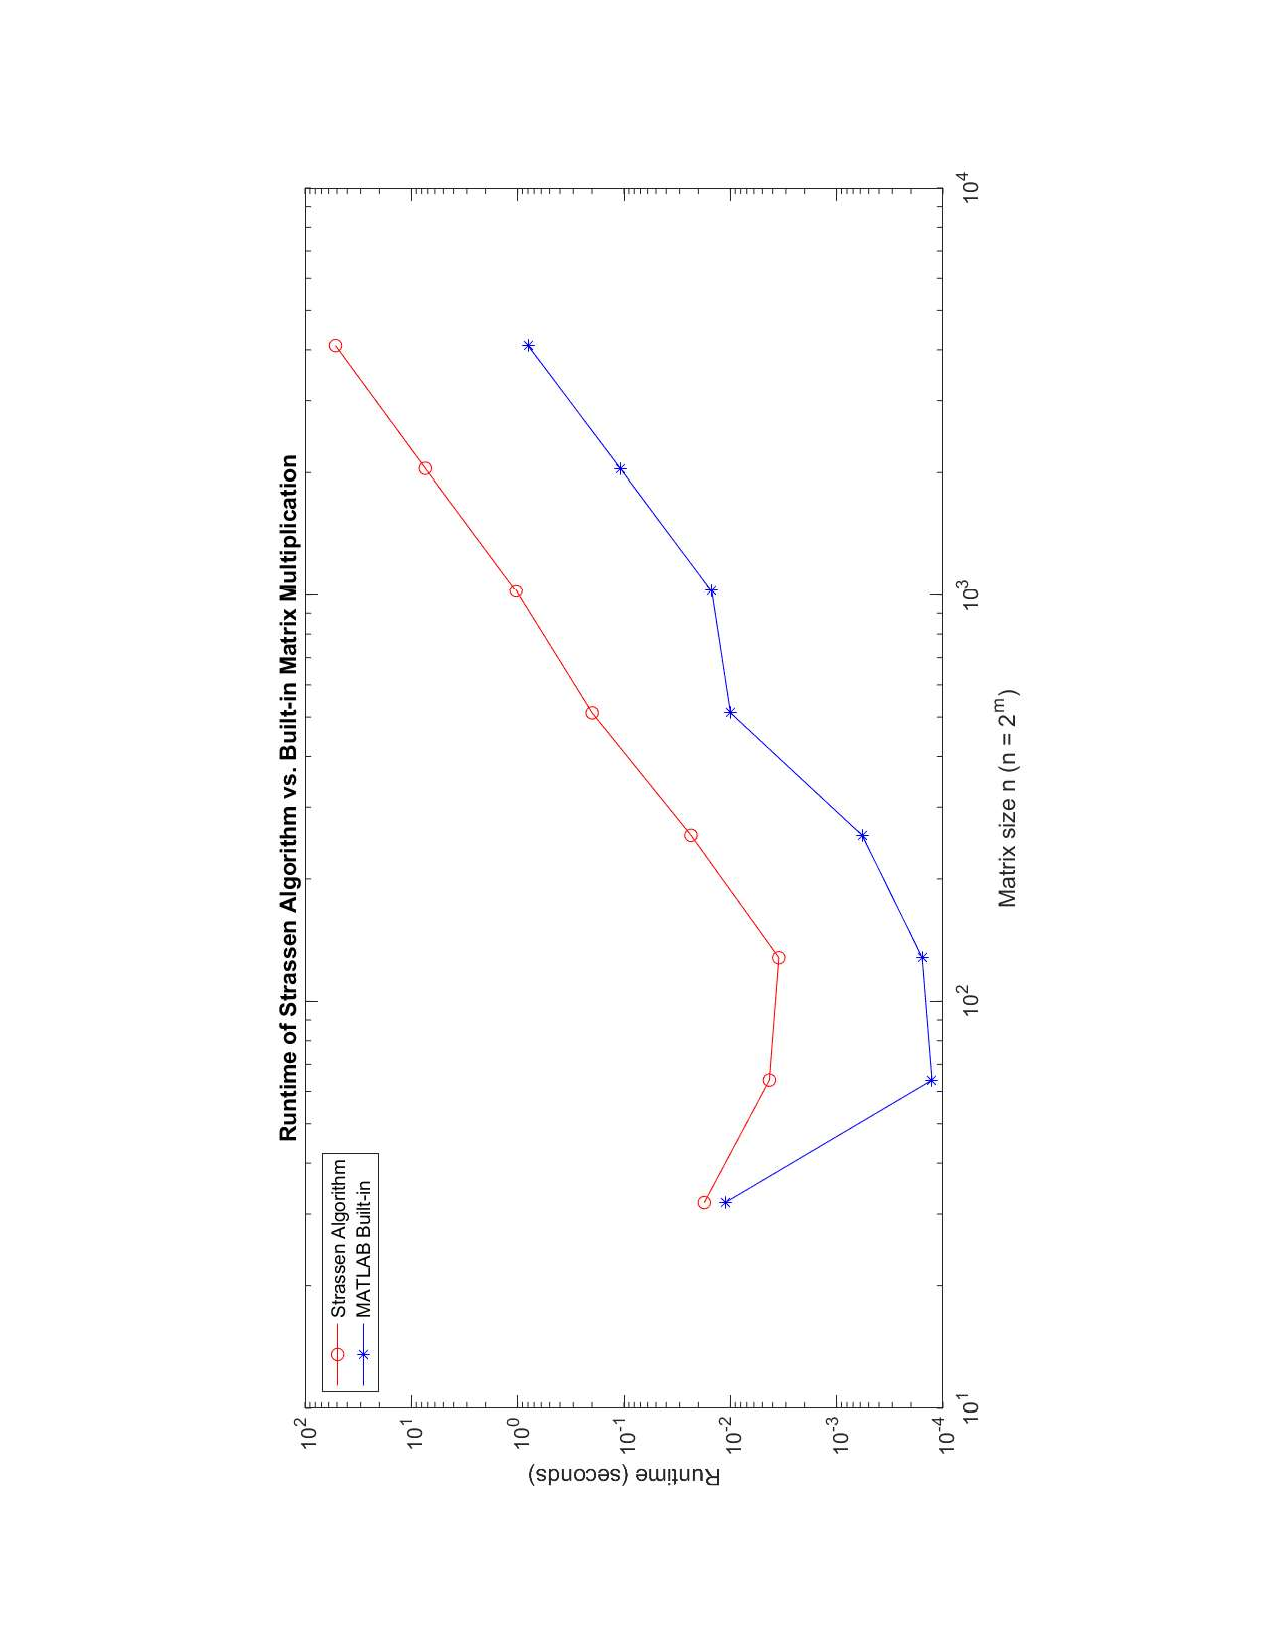
\includepdf[pages=-,scale=0.6,angle=270]{figure.pdf}
          \end{enumerate}
\end{enumerate}


\end{document}